\documentclass[11pt, letterpaper]{article}

% Fonts and Encoding
\usepackage[utf8]{inputenc}
\usepackage[T1]{fontenc}
\usepackage{lmodern} % High-quality Latin Modern vector font

% Math and Symbols
\usepackage{amsmath, amssymb, amsthm, amsfonts, mathrsfs, mathtools}

% Layout and Geometry (Adjusted for Landscape Cheat Sheet)
\usepackage{geometry}
\geometry{letterpaper, landscape, margin=0.5in}
\setlength{\parindent}{0pt}
\setlength{\parskip}{0.6em}

% Formatting and Graphics
\usepackage{graphicx, xcolor, enumitem, booktabs, array, tabularx, multicol}

% TikZ for Illustrations
\usepackage{tikz}
\usetikzlibrary{arrows.meta, positioning, shapes.geometric, calc, backgrounds, matrix}

% Clickable Links and TOC
\usepackage{hyperref}
\hypersetup{
    colorlinks=true,
    linkcolor=blue,
    filecolor=magenta,      
    urlcolor=cyan,
    pdftitle={Probability Distributions Cheat Sheet},
}

% Theorem Environments
\newtheorem{theorem}{Theorem}[section]
\newtheorem{lemma}[theorem]{Lemma}
\newtheorem{proposition}[theorem]{Proposition}
\newtheorem{corollary}[theorem]{Corollary}
\theoremstyle{definition}
\newtheorem{definition}{Definition}[section]
\newtheorem{axiom}{Axiom}[section]
\newtheorem{example}{Example}[section]
\theoremstyle{remark}
\newtheorem{remark}{Remark}[section]

% Custom Commands (Enforced standard notation)
\newcommand{\R}{\mathbb{R}}
\newcommand{\N}{\mathbb{N}}
\newcommand{\Z}{\mathbb{Z}}
\newcommand{\Q}{\mathbb{Q}}
\newcommand{\E}{\mathbb{E}}
\newcommand{\Prob}{\mathbb{P}}
\newcommand{\F}{\mathcal{F}}

\begin{document}

\title{\textbf{Probability Distributions Cheat Sheet}}
\author{Tashfeen Omran}
\date{\today}
\maketitle
\tableofcontents
\newpage

\section{Probability Distributions Summary}

\renewcommand{\arraystretch}{1.5}
\begin{tabularx}{\textwidth}{@{} l >{$\displaystyle}X<{$} >{$\displaystyle}c<{$} >{$\displaystyle}c<{$} >{$\displaystyle}c<{$} @{}}
\toprule
\textbf{Distribution} & \text{\textbf{PMF/PDF}} & \text{\textbf{E[Y]}} & \text{\textbf{Var[Y]}} & \text{\textbf{MGF}} \\
\midrule
\multicolumn{5}{@{}l}{\textbf{Discrete Distributions}} \\
\addlinespace[2pt]
Binomial & p(y) = \binom{n}{y} p^y (1-p)^{n-y} & np & np(1-p) & [pe^t + (1-p)]^n \\
Geometric & p(y) = p(1-p)^{y-1} & \frac{1}{p} & \frac{1-p}{p^2} & \frac{pe^t}{1-(1-p)e^t} \\
Hypergeometric & p(y) = \frac{\binom{r}{y}\binom{N-r}{n-y}}{\binom{N}{n}} & n\frac{r}{N} & n\left(\frac{r}{N}\right)\left(1-\frac{r}{N}\right)\left(\frac{N-n}{N-1}\right) & \text{--} \\
Poisson & p(y) = \frac{\lambda^y e^{-\lambda}}{y!} & \lambda & \lambda & \exp[\lambda(e^t - 1)] \\
Negative Binomial & p(y) = \binom{y-1}{r-1} p^r (1-p)^{y-r} & \frac{r}{p} & \frac{r(1-p)}{p^2} & \left[\frac{pe^t}{1-(1-p)e^t}\right]^r \\
\midrule
\multicolumn{5}{@{}l}{\textbf{Continuous Distributions}} \\
\addlinespace[2pt]
Uniform & f(y) = \frac{1}{\theta_2 - \theta_1}, \quad \theta_1 \le y \le \theta_2 & \frac{\theta_1 + \theta_2}{2} & \frac{(\theta_2 - \theta_1)^2}{12} & \frac{e^{t\theta_2} - e^{t\theta_1}}{t(\theta_2 - \theta_1)} \\
Normal & f(y) = \frac{1}{\sigma\sqrt{2\pi}}\exp\left[-\frac{(y-\mu)^2}{2\sigma^2}\right] & \mu & \sigma^2 & \exp\left(\mu t + \frac{t^2\sigma^2}{2}\right) \\
Exponential & f(y) = \frac{1}{\beta}e^{-y/\beta}, \quad \beta > 0 & \beta & \beta^2 & (1-\beta t)^{-1} \\
Gamma & f(y) = \frac{1}{\Gamma(\alpha)\beta^\alpha} y^{\alpha-1}e^{-y/\beta} & \alpha\beta & \alpha\beta^2 & (1-\beta t)^{-\alpha} \\
Chi-square & f(y) = \frac{y^{(\nu/2)-1}e^{-y/2}}{2^{\nu/2}\Gamma(\nu/2)} & \nu & 2\nu & (1-2t)^{-\nu/2} \\
Beta & f(y) = \frac{\Gamma(\alpha+\beta)}{\Gamma(\alpha)\Gamma(\beta)} y^{\alpha-1}(1-y)^{\beta-1} & \frac{\alpha}{\alpha+\beta} & \frac{\alpha\beta}{(\alpha+\beta)^2(\alpha+\beta+1)} & \text{--} \\
\bottomrule
\end{tabularx}

\vspace{1em}

\section{Tchebysheff's Theorem}
Let $Y$ be a random variable with mean $\mu$ and finite variance $\sigma^2$. For any constant $k > 0$:
\[ \Prob(|Y-\mu| < k\sigma) \ge 1 - \frac{1}{k^2} \quad \text{or} \quad \Prob(|Y-\mu| \ge k\sigma) \le \frac{1}{k^2} \]
\textbf{Proof using Markov's Inequality:} \\
Markov's Inequality states that for a non-negative random variable $X$ and $a > 0$, $\Prob(X \ge a) \le \frac{\E[X]}{a}$. \\
Let $X = (Y-\mu)^2$ and $a = k^2\sigma^2$. Then:
\[ \Prob(|Y-\mu| \ge k\sigma) = \Prob((Y-\mu)^2 \ge k^2\sigma^2) \le \frac{\E[(Y-\mu)^2]}{k^2\sigma^2} = \frac{\sigma^2}{k^2\sigma^2} = \frac{1}{k^2} \]

\vspace{1em}
\hrule
\vspace{1em}

\begin{multicols*}{2}

\section{Discrete Distributions}

\subsection{Binomial Distribution: $Y \sim \text{Binomial}(n, p)$}
\textbf{Example:} Out of 7 customized sandwiches, the probability of the customization being perfectly right is $0.3$. What is the formula for the probability that 3 or fewer are perfect? \\
\textbf{Formula:} $\sum_{y=0}^{3} \binom{7}{y} (0.3)^y (0.7)^{7-y}$

\textbf{Expected Value:} $\E[Y] = np$
\begin{align*}
\E[Y] &= \sum_{y=1}^{n} y \frac{n!}{y!(n-y)!} p^y q^{n-y} \\
&= np \sum_{y=1}^{n} \frac{(n-1)!}{(y-1)!(n-y)!} p^{y-1} q^{n-y} \\
&= np \sum_{k=0}^{n-1} \binom{n-1}{k} p^k q^{(n-1)-k} = np(p+q)^{n-1} = np
\end{align*}

\textbf{Variance:} $\text{Var}(Y) = np(1-p)$
\begin{align*}
\E[Y(Y-1)] &= \sum_{y=2}^{n} y(y-1) \binom{n}{y} p^y q^{n-y} \\
&= n(n-1)p^2 \sum_{y=2}^{n} \binom{n-2}{y-2} p^{y-2} q^{n-y} = n(n-1)p^2 \\
\text{Var}(Y) &= \E[Y(Y-1)] + \E[Y] - (\E[Y])^2 \\
&= n(n-1)p^2 + np - n^2p^2 = np(1-p)
\end{align*}

\textbf{MGF:} $\E[e^{tY}] = [pe^t + (1-p)]^n$
\begin{align*}
\E[e^{tY}] &= \sum_{y=0}^{n} e^{ty} \binom{n}{y} p^y q^{n-y} \\
&= \sum_{y=0}^{n} \binom{n}{y} (pe^t)^y q^{n-y} = (pe^t + q)^n
\end{align*}

\subsection{Geometric Distribution: $Y \sim \text{Geometric}(p)$}
\textbf{Example:} A server request fails with probability $0.5$. What is the formula for the probability it takes 3 or more requests to get the first success? \\
\textbf{Formula:} $\Prob(Y \ge 3) = (0.5)^{3-1} = 0.25$

\textbf{Expected Value:} $\E[Y] = \frac{1}{p}$
\begin{align*}
\E[Y] &= \sum_{y=1}^{\infty} y q^{y-1} p = p \frac{d}{dq} \left( \sum_{y=0}^{\infty} q^y \right) \\
&= p \frac{d}{dq} \left( \frac{1}{1-q} \right) = p \left( \frac{1}{(1-q)^2} \right) = \frac{1}{p}
\end{align*}

\textbf{Variance:} $\text{Var}(Y) = \frac{1-p}{p^2}$
\begin{align*}
\E[Y(Y-1)] &= \sum_{y=2}^{\infty} y(y-1) q^{y-1} p = pq \frac{d^2}{dq^2} \left( \sum_{y=0}^{\infty} q^y \right) \\
&= pq \left( \frac{2}{(1-q)^3} \right) = \frac{2q}{p^2} \\
\text{Var}(Y) &= \frac{2q}{p^2} + \frac{1}{p} - \frac{1}{p^2} = \frac{1-p}{p^2}
\end{align*}

\textbf{MGF:} $\E[e^{tY}] = \frac{pe^t}{1-(1-p)e^t}$
\begin{align*}
\E[e^{tY}] &= \sum_{y=1}^{\infty} e^{ty} q^{y-1} p = \frac{p}{q} \sum_{y=1}^{\infty} (qe^t)^y \\
&= \frac{p}{q} \left( \frac{qe^t}{1-qe^t} \right) = \frac{pe^t}{1-qe^t}
\end{align*}

\subsection{Hypergeometric Distribution: $Y \sim \text{Hypergeometric}(N, r, n)$}
\textbf{Example:} From 8 Papa John's slices, 4 have jalapeños. If you eat 4 slices, what is the formula for the probability exactly 2 have jalapeños? \\
\textbf{Formula:} $\frac{\binom{4}{2}\binom{4}{2}}{\binom{8}{4}}$

\textbf{Expected Value:} $\E[Y] = \frac{nr}{N}$
\begin{align*}
\E[Y] &= \sum_{y=1}^{n} y \frac{\binom{r}{y}\binom{N-r}{n-y}}{\binom{N}{n}} = \frac{r}{\binom{N}{n}} \sum_{y=1}^{n} \binom{r-1}{y-1}\binom{N-r}{n-y} \\
&= r \frac{\binom{N-1}{n-1}}{\binom{N}{n}} = \frac{nr}{N}
\end{align*}

\textbf{Variance:} $\text{Var}(Y) = n\left(\frac{r}{N}\right)\left(1-\frac{r}{N}\right)\left(\frac{N-n}{N-1}\right)$
\begin{align*}
\E[Y(Y-1)] &= \frac{r(r-1)}{\binom{N}{n}} \sum_{y=2}^{n} \binom{r-2}{y-2}\binom{N-r}{n-y} \\
&= r(r-1) \frac{\binom{N-2}{n-2}}{\binom{N}{n}} = \frac{r(r-1)n(n-1)}{N(N-1)} \\
\text{Var}(Y) &= \frac{r(r-1)n(n-1)}{N(N-1)} + \frac{nr}{N} - \left(\frac{nr}{N}\right)^2 \\
&= n\left(\frac{r}{N}\right)\left(1-\frac{r}{N}\right)\left(\frac{N-n}{N-1}\right)
\end{align*}

\subsection{Poisson Distribution: $Y \sim \text{Poisson}(\lambda)$}
\textbf{Example:} Your building's utility service goes out at an average rate of 6 times a year. What is the formula for the probability of strictly less than 2 outages this year? \\
\textbf{Formula:} $\Prob(Y < 2) = \frac{6^0 e^{-6}}{0!} + \frac{6^1 e^{-6}}{1!} = 7e^{-6}$

\textbf{Expected Value:} $\E[Y] = \lambda$
\begin{align*}
\E[Y] &= \sum_{y=1}^{\infty} y \frac{\lambda^y e^{-\lambda}}{y!} = \lambda e^{-\lambda} \sum_{y=1}^{\infty} \frac{\lambda^{y-1}}{(y-1)!} \\
&= \lambda e^{-\lambda} e^\lambda = \lambda
\end{align*}

\textbf{Variance:} $\text{Var}(Y) = \lambda$
\begin{align*}
\E[Y(Y-1)] &= \sum_{y=2}^{\infty} y(y-1) \frac{\lambda^y e^{-\lambda}}{y!} = \lambda^2 e^{-\lambda} \sum_{y=2}^{\infty} \frac{\lambda^{y-2}}{(y-2)!} = \lambda^2 \\
\text{Var}(Y) &= \lambda^2 + \lambda - \lambda^2 = \lambda
\end{align*}

\textbf{MGF:} $\E[e^{tY}] = \exp[\lambda(e^t - 1)]$
\begin{align*}
\E[e^{tY}] &= \sum_{y=0}^{\infty} e^{ty} \frac{\lambda^y e^{-\lambda}}{y!} = e^{-\lambda} \sum_{y=0}^{\infty} \frac{(\lambda e^t)^y}{y!} \\
&= e^{-\lambda} e^{\lambda e^t} = e^{\lambda(e^t - 1)}
\end{align*}

\subsection{Negative Binomial Distribution: $Y \sim \text{NB}(r, p)$}
\textbf{Example:} The probability a Topgolf swing clears 150 yards is $0.4$. What is the formula for the probability that the 3rd swing clearing 150 yards is exactly the 7th attempt? \\
\textbf{Formula:} $\binom{7-1}{3-1} (0.4)^3 (0.6)^{7-3}$

\textbf{Expected Value:} $\E[Y] = \frac{r}{p}$
\begin{align*}
\E[Y] &= \sum_{y=r}^{\infty} y \binom{y-1}{r-1} p^r q^{y-r} = r \sum_{y=r}^{\infty} \binom{y}{r} p^r q^{y-r} \\
&= \frac{r}{p} \sum_{w=r+1}^{\infty} \binom{w-1}{r} p^{r+1} q^{w-(r+1)} = \frac{r}{p}
\end{align*}

\textbf{Variance:} $\text{Var}(Y) = \frac{r(1-p)}{p^2}$
\begin{align*}
\E[Y(Y+1)] &= \sum_{y=r}^{\infty} y(y+1)\binom{y-1}{r-1}p^r q^{y-r} \\
&= r(r+1)\sum_{y=r}^{\infty} \binom{y+1}{r+1}p^r q^{y-r} = \frac{r(r+1)}{p^2} \\
\text{Var}(Y) &= \E[Y^2] - (\E[Y])^2 = \left(\E[Y(Y+1)] - \E[Y]\right) - (\E[Y])^2 \\
&= \frac{r^2+r}{p^2} - \frac{r}{p} - \frac{r^2}{p^2} = \frac{r(1-p)}{p^2}
\end{align*}

\textbf{MGF:} Sum of $r$ i.i.d. Geometric RVs.
\[ M_Y(t) = [M_{\text{Geo}}(t)]^r = \left(\frac{pe^t}{1-qe^t}\right)^r \]

\section{Continuous Distributions}

\subsection{Uniform Distribution: $Y \sim U(\theta_1, \theta_2)$}
\textbf{Example:} [Insert Uniform Distribution Example Here] \\
\textbf{Formula:} [Insert Formula Here]

\textbf{Expected Value:} $\E[Y] = \frac{\theta_1 + \theta_2}{2}$
\begin{align*}
\E[Y] &= \int_{\theta_1}^{\theta_2} \frac{y}{\theta_2 - \theta_1} dy = \frac{1}{\theta_2 - \theta_1} \left[ \frac{y^2}{2} \right]_{\theta_1}^{\theta_2} = \frac{\theta_1 + \theta_2}{2}
\end{align*}

\textbf{Variance:} $\text{Var}(Y) = \frac{(\theta_2 - \theta_1)^2}{12}$
\begin{align*}
\E[Y^2] &= \int_{\theta_1}^{\theta_2} \frac{y^2}{\theta_2 - \theta_1} dy = \frac{\theta_2^3 - \theta_1^3}{3(\theta_2 - \theta_1)} = \frac{\theta_1^2 + \theta_1\theta_2 + \theta_2^2}{3} \\
\text{Var}(Y) &= \frac{\theta_1^2 + \theta_1\theta_2 + \theta_2^2}{3} - \frac{(\theta_1 + \theta_2)^2}{4} = \frac{(\theta_2 - \theta_1)^2}{12}
\end{align*}

\textbf{MGF:} $\E[e^{tY}] = \frac{e^{t\theta_2} - e^{t\theta_1}}{t(\theta_2 - \theta_1)}$
\begin{align*}
\E[e^{tY}] &= \int_{\theta_1}^{\theta_2} \frac{e^{ty}}{\theta_2 - \theta_1} dy = \frac{1}{t(\theta_2 - \theta_1)} \left[ e^{ty} \right]_{\theta_1}^{\theta_2} = \frac{e^{t\theta_2} - e^{t\theta_1}}{t(\theta_2 - \theta_1)}
\end{align*}

\subsection{Normal Distribution: $Y \sim N(\mu, \sigma^2)$}
\textbf{Example:} [Insert Normal Distribution Example Here] \\
\textbf{Formula:} [Insert Formula Here]

\begin{center}
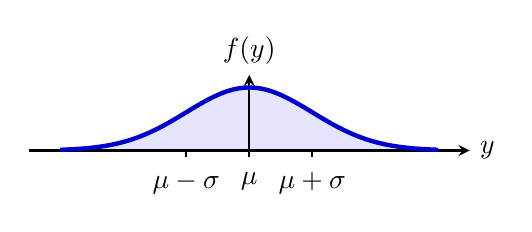
\begin{tikzpicture}[scale=0.8]
    % 1) Backgrounds
    \fill[blue!10] (-2.5,0) -- plot[domain=-2.5:2.5, samples=50] (\x, {exp(-0.5*\x*\x)}) -- (2.5,0) -- cycle;
    % 2) Grid/Axes
    \draw[->, >=stealth, thick] (-3.5,0) -- (3.5,0) node[right] {$y$};
    \draw[->, >=stealth, thick] (0,0) -- (0,1.2) node[above] {$f(y)$};
    % 3) Primary plots
    \draw[ultra thick, blue!80!black, domain=-3:3, samples=100] plot (\x, {exp(-0.5*\x*\x)});
    % 4) Nodes/Labels
    \draw[thick] (0,0) -- (0,-0.1) node[below=2pt] {$\mu$};
    \draw[thick] (1,0) -- (1,-0.1) node[below=2pt] {$\mu+\sigma$};
    \draw[thick] (-1,0) -- (-1,-0.1) node[below=2pt] {$\mu-\sigma$};
\end{tikzpicture}
\end{center}

\textbf{Expected Value:} $\E[Y] = \mu$ \\
Let $z = \frac{y-\mu}{\sigma} \implies y = \sigma z + \mu, \, dy = \sigma dz$:
\begin{align*}
\E[Y] &= \int_{-\infty}^{\infty} (\sigma z + \mu) \frac{1}{\sqrt{2\pi}} e^{-z^2/2} dz \\
&= \sigma \int_{-\infty}^{\infty} \frac{z}{\sqrt{2\pi}} e^{-z^2/2} dz + \mu \int_{-\infty}^{\infty} \frac{1}{\sqrt{2\pi}} e^{-z^2/2} dz \\
&= \sigma(0) + \mu(1) = \mu
\end{align*}

\textbf{Variance:} $\text{Var}(Y) = \sigma^2$
\begin{align*}
\text{Var}(Y) &= \int_{-\infty}^{\infty} (y-\mu)^2 f(y) dy = \sigma^2 \int_{-\infty}^{\infty} z^2 \frac{1}{\sqrt{2\pi}} e^{-z^2/2} dz \\
&= \frac{\sigma^2}{\sqrt{2\pi}} \left( \left[-z e^{-z^2/2}\right]_{-\infty}^{\infty} + \int_{-\infty}^{\infty} e^{-z^2/2} dz \right) = \sigma^2
\end{align*}

\textbf{MGF:} $\E[e^{tY}] = \exp\left(\mu t + \frac{t^2\sigma^2}{2}\right)$
\begin{align*}
\E[e^{tY}] &= \int_{-\infty}^{\infty} e^{ty} \frac{1}{\sigma\sqrt{2\pi}} e^{-\frac{(y-\mu)^2}{2\sigma^2}} dy \quad \text{Let } y = z\sigma + \mu \\
&= e^{\mu t} \int_{-\infty}^{\infty} \frac{1}{\sqrt{2\pi}} e^{-\frac{1}{2}(z^2 - 2t\sigma z)} dz \\
&= e^{\mu t + \frac{1}{2}t^2\sigma^2} \int_{-\infty}^{\infty} \frac{1}{\sqrt{2\pi}} e^{-\frac{1}{2}(z - t\sigma)^2} dz = e^{\mu t + \frac{1}{2}t^2\sigma^2}
\end{align*}

\subsection{Exponential Distribution: $Y \sim \text{Exp}(\beta)$}
\textbf{Example:} [Insert Exponential Distribution Example Here] \\
\textbf{Formula:} [Insert Formula Here]

\textbf{Expected Value:} $\E[Y] = \beta$
\begin{align*}
\E[Y] &= \int_{0}^{\infty} y \frac{1}{\beta} e^{-y/\beta} dy = \left[ -y e^{-y/\beta} \right]_{0}^{\infty} + \int_{0}^{\infty} e^{-y/\beta} dy = \beta
\end{align*}

\textbf{Variance:} $\text{Var}(Y) = \beta^2$
\begin{align*}
\E[Y^2] &= \int_{0}^{\infty} y^2 \frac{1}{\beta} e^{-y/\beta} dy = \left[ -y^2 e^{-y/\beta} \right]_{0}^{\infty} + 2\beta \int_{0}^{\infty} \frac{y}{\beta} e^{-y/\beta} dy \\
&= 2\beta \E[Y] = 2\beta^2 \\
\text{Var}(Y) &= 2\beta^2 - \beta^2 = \beta^2
\end{align*}

\textbf{MGF:} $\E[e^{tY}] = (1-\beta t)^{-1}$
\begin{align*}
\E[e^{tY}] &= \int_{0}^{\infty} \frac{1}{\beta} e^{-y\left(\frac{1}{\beta}-t\right)} dy = \frac{1}{\beta\left(\frac{1}{\beta}-t\right)} = \frac{1}{1-\beta t}
\end{align*}

\subsection{Gamma Distribution: $Y \sim \text{Gamma}(\alpha, \beta)$}
\textbf{Example:} [Insert Gamma Distribution Example Here] \\
\textbf{Formula:} [Insert Formula Here]

\textbf{Expected Value:} $\E[Y] = \alpha\beta$
\begin{align*}
\E[Y] &= \int_{0}^{\infty} y \frac{y^{\alpha-1} e^{-y/\beta}}{\beta^\alpha \Gamma(\alpha)} dy = \frac{\beta^{\alpha+1} \Gamma(\alpha+1)}{\beta^\alpha \Gamma(\alpha)} = \alpha\beta
\end{align*}

\textbf{Variance:} $\text{Var}(Y) = \alpha\beta^2$
\begin{align*}
\E[Y^2] &= \int_{0}^{\infty} y^2 \frac{y^{\alpha-1} e^{-y/\beta}}{\beta^\alpha \Gamma(\alpha)} dy = \frac{\beta^{\alpha+2} \Gamma(\alpha+2)}{\beta^\alpha \Gamma(\alpha)} = \alpha(\alpha+1)\beta^2 \\
\text{Var}(Y) &= \alpha(\alpha+1)\beta^2 - (\alpha\beta)^2 = \alpha\beta^2
\end{align*}

\textbf{MGF:} $\E[e^{tY}] = (1-\beta t)^{-\alpha}$
\begin{align*}
\E[e^{tY}] &= \int_{0}^{\infty} \frac{y^{\alpha-1} e^{-y(1/\beta - t)}}{\beta^\alpha \Gamma(\alpha)} dy \quad \text{Let } u = \frac{1}{\beta} - t \\
&= \frac{1}{\beta^\alpha \Gamma(\alpha)} \int_{0}^{\infty} y^{\alpha-1} e^{-yu} dy = \frac{u^{-\alpha} \Gamma(\alpha)}{\beta^\alpha \Gamma(\alpha)} = (1-\beta t)^{-\alpha}
\end{align*}

\subsection{Chi-Square Distribution: $Y \sim \chi^2(\nu)$}
\textbf{Example:} [Insert Chi-Square Distribution Example Here] \\
\textbf{Formula:} [Insert Formula Here]

Special case of Gamma with $\alpha = \nu/2$ and $\beta = 2$.
\begin{align*}
\E[Y] &= \alpha\beta = \left(\frac{\nu}{2}\right)(2) = \nu \\
\text{Var}(Y) &= \alpha\beta^2 = \left(\frac{\nu}{2}\right)(2)^2 = 2\nu \\
\E[e^{tY}] &= (1-\beta t)^{-\alpha} = (1-2t)^{-\nu/2}
\end{align*}

\subsection{Beta Distribution: $Y \sim \text{Beta}(\alpha, \beta)$}
\textbf{Example:} [Insert Beta Distribution Example Here] \\
\textbf{Formula:} [Insert Formula Here]

\textbf{Expected Value:} $\E[Y] = \frac{\alpha}{\alpha+\beta}$
\begin{align*}
\E[Y] &= \int_{0}^{1} y \frac{y^{\alpha-1} (1-y)^{\beta-1}}{B(\alpha, \beta)} dy = \frac{B(\alpha+1, \beta)}{B(\alpha, \beta)} = \frac{\alpha}{\alpha+\beta}
\end{align*}

\textbf{Variance:} $\text{Var}(Y) = \frac{\alpha\beta}{(\alpha+\beta)^2(\alpha+\beta+1)}$
\begin{align*}
\E[Y^2] &= \frac{B(\alpha+2, \beta)}{B(\alpha, \beta)} = \frac{\alpha(\alpha+1)}{(\alpha+\beta)(\alpha+\beta+1)} \\
\text{Var}(Y) &= \frac{\alpha(\alpha+1)}{(\alpha+\beta)(\alpha+\beta+1)} - \left(\frac{\alpha}{\alpha+\beta}\right)^2 \\
&= \frac{\alpha\beta}{(\alpha+\beta)^2(\alpha+\beta+1)}
\end{align*}

\end{multicols*}
\end{document}